%!TEX root = main.tex

\section{Problem formulation}
\label{sec:system-model}

\subsection{Route flow estimation}
The route flow estimation problem (illustrated in Fig.~\ref{fig:example-setup}) is as follows: for a road network $G=(V,E)$, let $\mathcal{R}$ denote the set of $n$ routes that vehicles take.  The route flow $x \in \mathbb{R}^n$ is the unknown state of the road network.  We employ sensor measurments cellpath flow $f$, origin-destination (OD) flow $d$, and link flow $b$.  We are given the linear operators $U, T, A$ relating the sensor measurements to the route flow $x$, that is, $Ax=b, Tx=d, Ux=f$. We wish to estimate the state $x$ from the sensor data $f,d,b$.

With the exception of the noise model, we follow the same assumptions as in \cite{Wu2015}: static setting, and continuous and well-posed cellpaths.

\begin{figure}[htb]
  \centering
    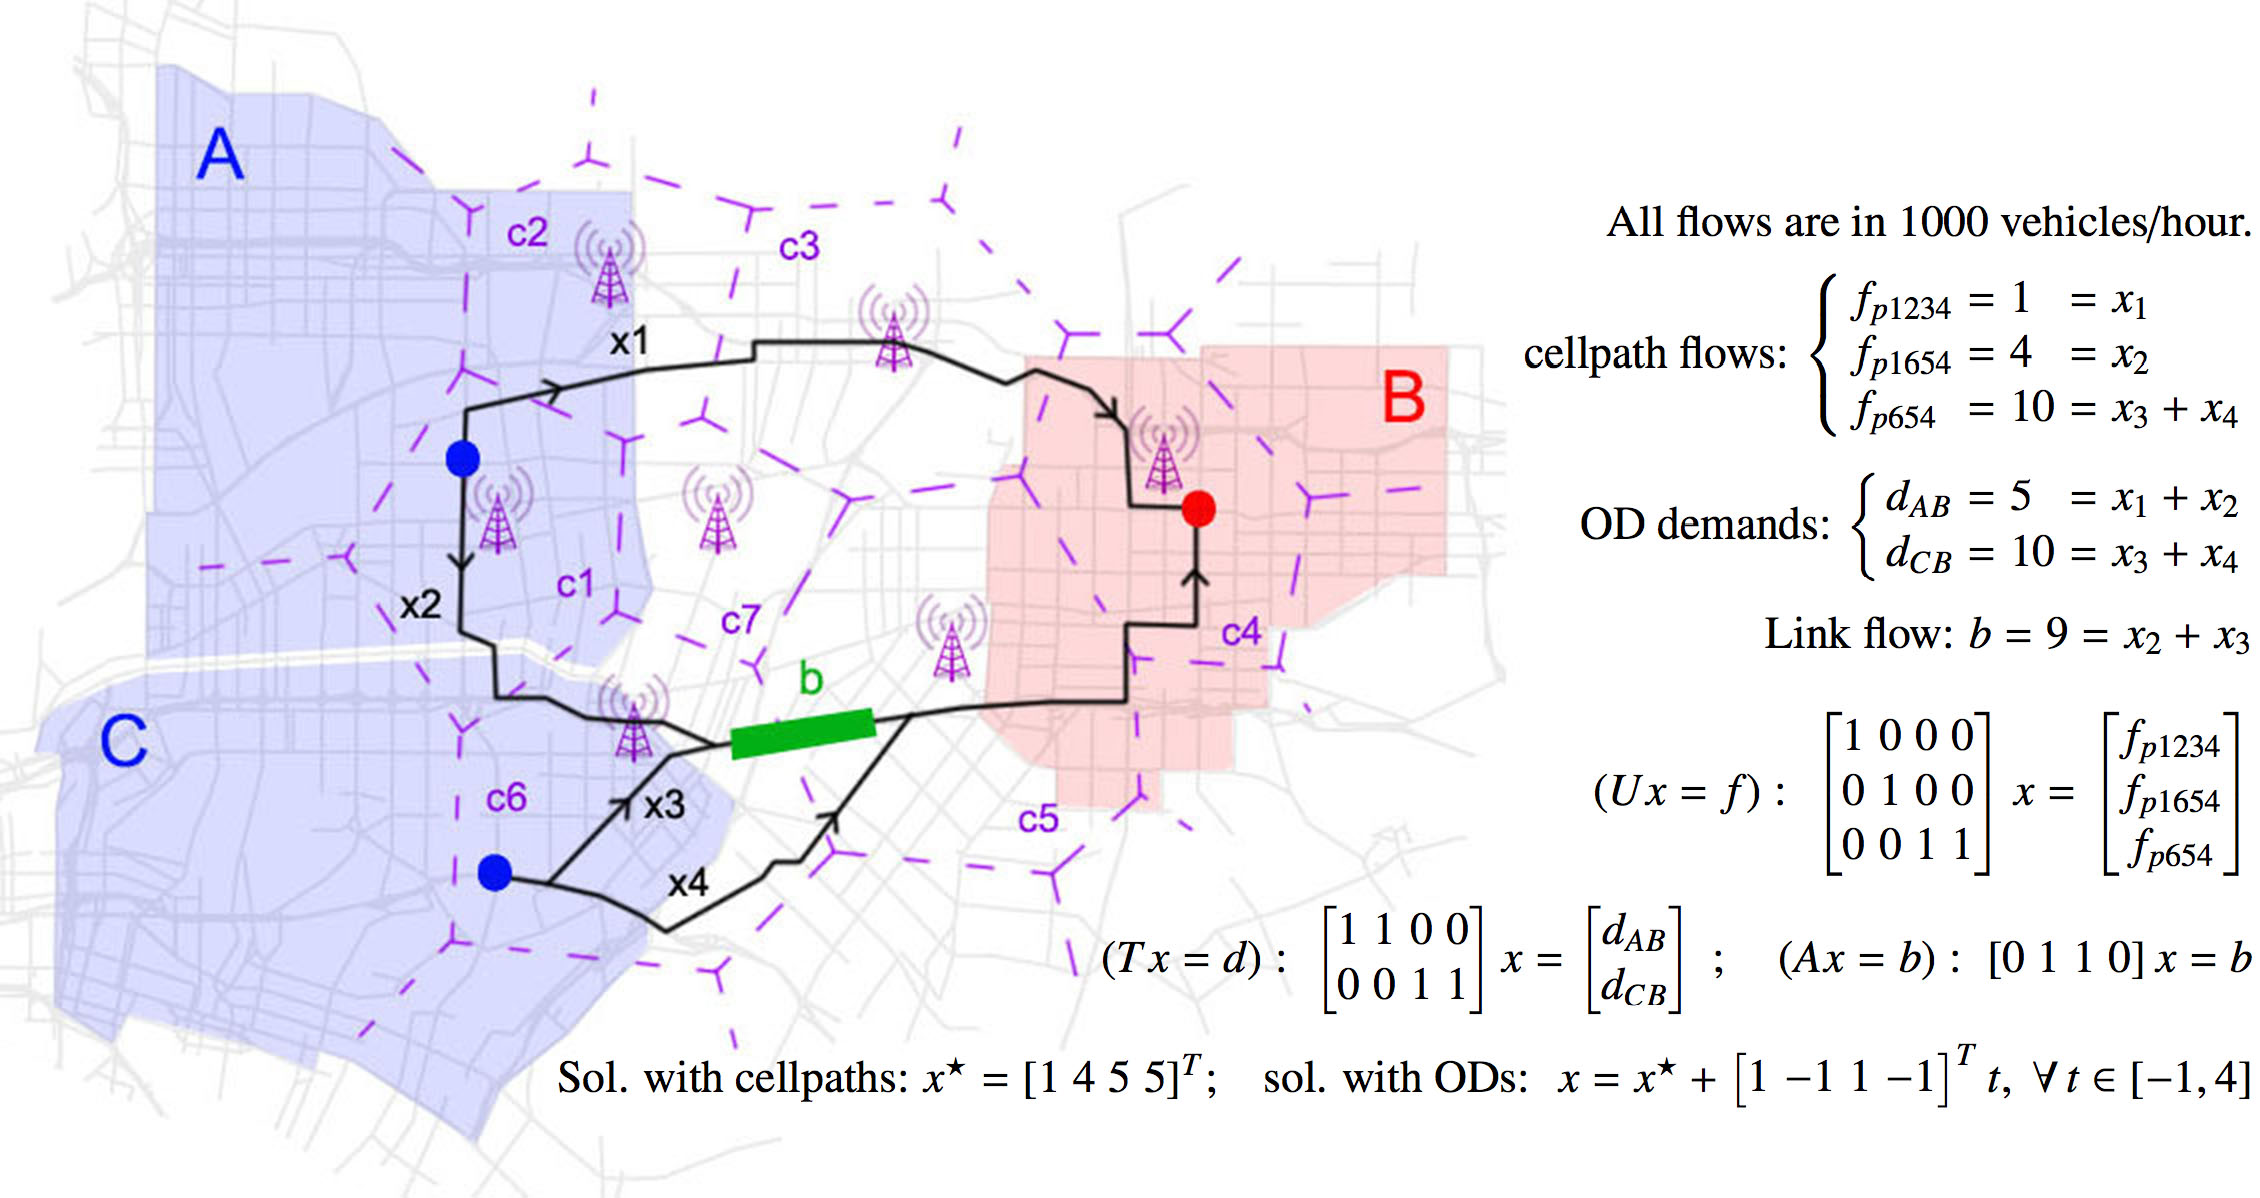
\includegraphics[width=0.47	\textwidth]{figures/setup}
  \caption{\footnotesize{In this illustration, we have two origins A and C ({\color{blue}blue}) and one destination B ({\color{red}red}). We have routes $r_1,r_2,r_3,r_4$ with flows $x=(x_1,x_2,x_3, x_4)$ such that $r_1,r_2$ go from A to B and $r_3,r_4$ go from C to B. Cells $c_1,\cdots,c_7$ are shown in {\color{magenta} purple} dashed regions. Since route $r_1$ goes through cells $c_1,c_2,c_3,c_4$, its associated cellpath is $p_{1234}$. Similarly, routes $r_2,r_3,r_4$ have cellpaths $p_{1654},p_{654},p_{654}$ respectively. Let $f_{p1234},\,f_{p1654},\,f_{p654}$ be the cellpath flows (obtained from cellular network data), \emph{i.e.} there are $f_{p1234}$=1000~veh/h going through $c_1,c_2,c_3,c_4$. Let $d_{AB}$ and $d_{CB}$ be the OD demands and $b$ be the link flow ({\color{green}green}, from loop detectors). Without considering data from cellpaths, the problem has \emph{one degree of freedom} and is \emph{underdetermined} with only the OD demands as data.}}
  \label{fig:example-setup}
\end{figure}

\subsection{Cell tower handoff noise model}

This work models the assignment of individual vehicles to cell towers with an effective received signal strength (eRSS) based decision process.  This eRSS between a vehicle $v$ and a cell tower $t$ is calculated from the received power by introducing tower handoff dynamics as noise penalties;
each vehicle gets assigned to the cell tower with the highest eRSS value at each time point in the simulation.

The actual received signal strength is attenuated by two sources: the path loss $P_d$ is a function of the distance between the vehicle and the cell tower $d_{v-t}$ and path loss exponent $\gamma$, while 
interference, multipath effects, and other RF noise are wrapped up into a uniformly distributed random penalty $P_{int}$.

The dynamics of the tower handoff, $P_{handoff}$, are modelled using two parameters.  $P_{hyst}$ represents hysteresis in the system by boosting the eRSS of the currently associated tower, biasing individual vehicles against switching towers.  $P_{load}$ represents the load balancing efforts to distribute usage across the cell network, adding an eRSS penalty to heavily loaded towers proportional to $N_t$, the number of other vehicles already connected to tower $t$.  

The eRSS can then be calculated as a function of the parameter vector $\phi = \{$interference, hysteresis, load balancing$\} = \{\alpha/\gamma, \beta/\gamma, \xi/\gamma\}$ over which we conduct our sensitivity analysis, evaluating the relative impacts of handoff dynamics in the presence of RF noise on route flow estimation.

\begin{eqnarray}
  eRSS_{v-t} & = & \left( \frac{P_{RX_v}}{P_{TX_t}} \right)_{dB} 
                   + P_{handoff_{v-t}} \\
  & = & P_{d_{v-t}} +P_{int} + P_{hyst_{v-t}} + P_{load_t}, \\
  P_{d_{v-t}} & = & -10 \gamma \log_{10} d_{v-t}, \\
  P_{int} & = & -\alpha \cdot \mathrm{Unif}(0,1). \\
  P_{hyst_{v-t}} & = & \begin{dcases}
    \beta & \mathrm{if~} v \mathrm{~is~already~connected~to~} t, \\
    0 & \mathrm{otherwise,}
  \end{dcases} \\
  P_{load_t} & = & -\xi \cdot N_{t}.
\end{eqnarray}

\subsection{Limitations}
  
In this work, we only consider hard handoffs, wherein each vehicle is connected to exactly one cell tower at all times.  The load balancing is represented by a linear penalty on tower utilization, which ignores nonlinear effects such as maximum tower capacity.  The units are arbitrarily scaled, and so require manual tuning to determine appropriate relative weights.
